\documentclass{article}

\usepackage{pgfplots}
\usepackage{amsmath}
\usepackage[margin=1in]{geometry}
\usepackage{subcaption}

\pgfplotsset{compat=1.18}

\begin{document}

\begin{figure}[t]
\centering

% -------- (a) Graph 1 --------
\begin{subfigure}[t]{0.48\textwidth}
\centering
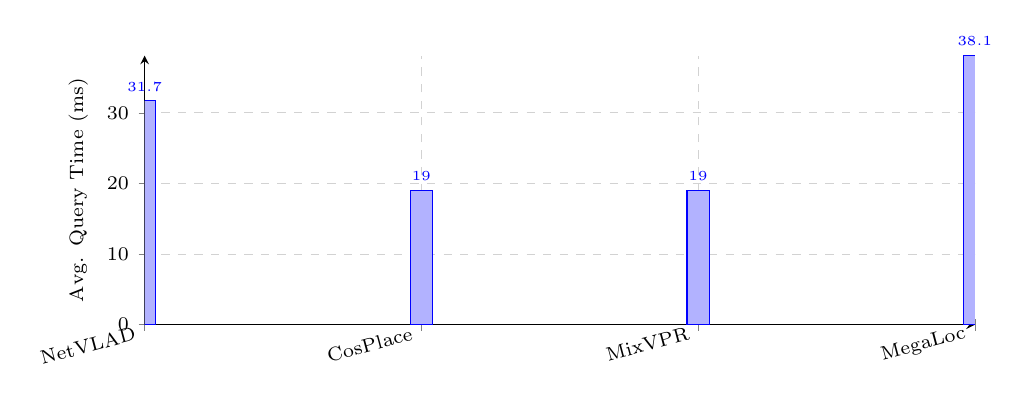
\begin{tikzpicture}
\begin{axis}[
    ybar,
    bar width=8pt,
    width=\textwidth,
    height=5cm,
    ymin=0,
    ylabel={Avg. Query Time (ms)},
    symbolic x coords={NetVLAD, CosPlace, MixVPR, MegaLoc},
    xtick=data,
    xticklabel style={rotate=15, anchor=east},
    tick label style={font=\scriptsize},
    label style={font=\scriptsize},
    nodes near coords,
    nodes near coords style={font=\tiny},
    grid=major,
    major grid style={dashed, gray!35},
    axis lines=left
]
\addplot coordinates {
    (NetVLAD, 31.7)
    (CosPlace, 19.0)
    (MixVPR, 19.0)
    (MegaLoc, 38.1)
};
\end{axis}
\end{tikzpicture}
\caption{VPR only}
\end{subfigure}
\hfill

% -------- (b) Graph 2 --------
\begin{subfigure}[t]{0.48\textwidth}
\centering
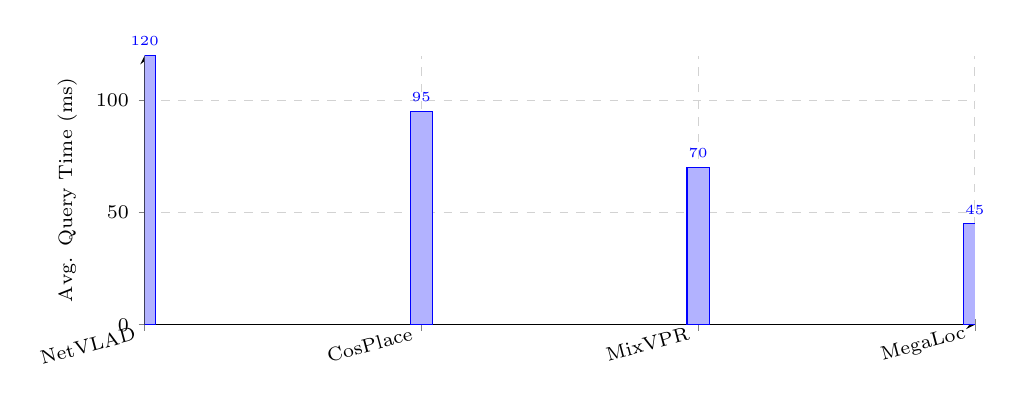
\begin{tikzpicture}
\begin{axis}[
    ybar,
    bar width=8pt,
    width=\textwidth,
    height=5cm,
    ymin=0,
    ylabel={Avg. Query Time (ms)},
    symbolic x coords={NetVLAD, CosPlace, MixVPR, MegaLoc},
    xtick=data,
    xticklabel style={rotate=15, anchor=east},
    tick label style={font=\scriptsize},
    label style={font=\scriptsize},
    nodes near coords,
    nodes near coords style={font=\tiny},
    grid=major,
    major grid style={dashed, gray!35},
    axis lines=left
]
\addplot coordinates {
    (NetVLAD, 120)
    (CosPlace, 95)
    (MixVPR, 70)
    (MegaLoc, 45)
};
\end{axis}
\end{tikzpicture}
\caption{VPR + Matching}
\end{subfigure}

\caption{Average query processing time comparison on the Tokyo dataset.}
\label{fig:query_time_comparison}

\end{figure}

\end{document}
